\documentclass[a4paper, 12pt]{article}
\usepackage{fullpage}

\usepackage{amsmath}
\usepackage{amssymb}
\usepackage{amsfonts}
\usepackage{amsthm}
\usepackage{mathtools}
\usepackage{soul}
\usepackage{hyperref}

\usepackage{color}
\usepackage{listings}

\definecolor{mygreen}{rgb}{0.0, 0.5, 0.0}
\definecolor{emphamber}{rgb}{1.0, 0.75, 0.0}
\definecolor{amber}{rgb}{1.0, 0.49, 0.0}
\definecolor{ballblue}{rgb}{0.13, 0.67, 0.8}
\definecolor{gray}{rgb}{0.5, 0.5, 0.5}

\lstdefinestyle{kamyarStyle}{
    basicstyle=\footnotesize\ttfamily,
    keywordstyle=\color{amber},
    stringstyle=\color{mygreen},
    commentstyle=\color{gray},
    breakatwhitespace=false,
    breaklines=true,
    keepspaces=true,
    showspaces=false,
    showstringspaces=false,
    showtabs=false,
}

\lstset{style=kamyarStyle}
\lstset{escapeinside={(*@}{@*)}}

\hypersetup{colorlinks=true, urlcolor=cyan}

\usepackage{xepersian}

\settextfont{XB Zar}
\ExplSyntaxOn \cs_set_eq:NN \etex_iffontchar:D \tex_iffontchar:D \ExplSyntaxOff
\setmathdigitfont{Yas}

\theoremstyle{definition}
\newtheorem{solution}{پاسخ}[section]
\newtheorem{solutionsection}{مورد}[solution]
\renewcommand{\thesolution}{\arabic{solution}}

\renewcommand{\baselinestretch}{1.3}

\definecolor{OliveGreen}{rgb}{0.84,1,0.64}

\begin{document}

\textbf{حسابگری زیستی؛}

\textbf{پیاده‌سازی شبکه عصبی؛}

\textbf{کامیار میرزاوزیری؛ 610396152}

\hrulefill

\tableofcontents

\newpage

\section{مقدمات و ابزارها}

مواردی که در این بخش به آن‌ها می‌پردازیم در فایل
\texttt{utils.py}
پیاده‌سازی شده‌اند.

همچنین تمام کدهای مربوط به این پروژه در مخزن گیت زیر موجود می‌باشد.

\begin{center}
    \url{https://github.com/kmirzavaziri/neural-network}
\end{center}

\subsection{توابع کمکی}
در پیاده‌سازی این پروژه به تعدادی توابع کمکی نیاز خواهیم داشت که همه آن‌ها را در کلاسی به اسم
\texttt{helpers}
پیاده‌سازی می‌کنیم.

در پیاده‌سازی محاسبات نورون‌ها به توابع
\texttt{sigmoid}
برای مشاهده شماره ۵، و
\texttt{softmax}
برای محاسبات لایه آخر
نیاز خواهیم داشت. این توابع را به صورت زیر پیاده‌سازی می‌کنیم.

\LTR
\begin{lstlisting}[language=Python]
def sigmoid(x):
    return 1 / (1 + np.exp(-np.array(x)))

def softmax(x):
    return np.exp(x) / np.sum(np.exp(x))
\end{lstlisting}
\RTL

همچنین نیاز داریم تا خطا را بر اساس فرمولی که در صورت پروژه داده شده محاسبه کنیم که برای این کار نیز تابع کمکی زیر را در نظر می‌گیریم.

\LTR
\begin{lstlisting}[language=Python]
def loss(y, nno):
    return -sum([np.log(nno[n][y[n]]) for n in range(len(y))]) / len(y)
\end{lstlisting}
\RTL

این تابع خروجی شبکه عصبی که برداری از احتمالات است را به همراه پاسخ درست دریافت می‌کند و برای هر مورد، احتمالی که شبکه عصبی برای پاسخ درست خروجی داده را در نظر می‌گیرد و لگاریتم این مقادیر را جمع می‌زند که با توجه به علامت منفی باعث می‌شود هرچه مقدار
\texttt{loss}
کم‌تر باشد، پاسخ بهتری داشته باشیم.

در نهایت دو تابع کمکی برای ایجاد داده‌ها از طریق کتابخانه
\texttt{sklearn}
ایجاد می‌کنیم. یکی از این توابع همان داده‌های موجود در صورت پروژه یعنی
\texttt{make\_moons}
و دیگری داده‌هایی با سه کلاس برای مشاهده شماره ۶ را خروجی می‌دهد. این توابع قادرند مجموعه داده‌های دریافت‌شده از کتابخانه
\texttt{sklearn}
را به دو بخش
\texttt{train}
و
\texttt{test}
بشکنند تا بتوانیم قدرت مدل شبکه عصبی را به درستی اندازه‌گیری کنیم.

\LTR
\begin{lstlisting}[language=Python]
def dataset(n, m):
    np.random.seed(0)
    x, y = datasets.make_moons(n + m, noise=0.20)
    return x[:n], y[:n], x[n:], y[n:]

def dataset_3(n, m):
    np.random.seed(0)
    x, y = datasets.make_classification(n + m, 2, n_classes=3, n_redundant=0, n_clusters_per_class=1)
    return x[:n], y[:n], x[n:], y[n:]
\end{lstlisting}
\RTL

\subsection{ترسیم‌گر}
کلاسی به اسم
\texttt{Visualizer}
پیاده‌سازی می‌کنیم که وظیفه ترسیم داده‌ها و کلاس‌های آن‌ها را دارد. این کلاس از کتابخانه
\texttt{matplotlib}
برای ترسیم استفاده می‌کند و کد آن در فایل
\texttt{utils.py}
موجود است اما چون مربوط به موضوع پروژه نمی‌باشد به آن نمی‌پردازیم.

\subsection{نورون}
می‌دانیم یک شبکه عصبی شامل تعدادی لایه است که در هر لایه تعدادی نورون وجود دارد. پس کلاسی به اسم
\texttt{Neuron}
برای پیاده‌سازی نورون‌ها که همان واحدهای محاسباتی شبکه عصبی می‌باشند تعریف می‌کنیم.

این کلاس ساده تنها شامل دو متد می‌باشد. متد اول که برای مقداردهی نورون به کار می‌رود تنها تعداد ورودی‌های نورون را به عنوان ورودی دریافت می‌کند. و دو بردار
\texttt{w}
و
\texttt{b}
را به طول تعداد ورودی‌های نورون تعریف می‌کند.

\LTR
\begin{lstlisting}[language=Python]
def __init__(self, input_size):
    self.input_size = input_size
    self.w = list(np.random.randn(self.input_size))
    self.b = [0.0] * self.input_size
\end{lstlisting}
\RTL

همانطور که می‌بینیم مقدار بردار
\texttt{b}
را در ابتدا صفر و مقدار بردار
\texttt{w}
را مقادیر تصادفی با توزیع نرمال در نظر می‌گیریم.

متد دیگر موظف است سیگنال ورودی به نورون که یک بردار به طول تعداد ورودی‌های نورون است را بگیرد و با توجه به بردارهای
\texttt{w}
و
\texttt{b}
و به کمک فرمول زیر، حاصل جمع این مقادیر را خروجی بدهد.

\[ \sum_{i = 0}^{\texttt{input\_size} - 1} x_i w_i + b_i. \]

\LTR
\begin{lstlisting}[language=Python]
def summation(self, signal):
    return sum([signal[i] * self.w[i] + self.b[i] for i in range(self.input_size)])
\end{lstlisting}
\RTL

\subsection{شبکه عصبی}
برای پیاده‌سازی شبکه عصبی، کلاسی به اسم
\texttt{NeuralNetwork}
تعریف می‌کنیم. از این کلاس انتظار داریم تا با دریافت یک سیگنال ورودی، سیگنالی را خروجی بدهد، و همچنین بتوانیم با داده‌هایی که پاسخ آن‌ها را از قبل می‌دانیم، آن را آموزش دهیم. پس دو متد اساسی
\texttt{compute}
و
\texttt{train}
باید روی این کلاس تعریف شده باشد. اما تعدادی توابع کمکی نیز برای سادگی کار روی این کلاس تعریف کرده‌ایم که در ادامه هر یک از این توابع را بررسی می‌کنیم.

\subsubsection{مقداردهی اولیه}
ابتدا لازم است پارامترهایی را در نظر بگیریم و با توجه به این پارامترها شبکه عصبی را راه‌اندازی کنیم. شبکه عصبی را طوری پیاده‌سازی می‌کنیم که موارد زیر همگی قابل تنظیم باشند.

\begin{itemize}
    \item تعداد لایه‌ها و تعداد نورون‌ها در هر لایه
    \item درجه یادگیری $\epsilon$
    \item قدرت تنظیم $\lambda$
    \item سایز دسته‌ها در \lr{\texttt{gradient descent}}
    \item درجه تبرید
    \item تابع فعال‌سازی
\end{itemize}

با این قابلیت انعطاف برای شبکه عصبی می‌توانیم تمام مشاهداتی که در صورت پروژه خواسته شده را به سادگی انجام دهیم. تعداد لایه‌ها و تعداد نورون‌های هر لایه را به صورت یک لیست از اعداد ورودی می‌گیریم که هر درایه آن تعداد نورون‌های آن لایه را نشان می‌دهد و بدیهتا درایه اول نشان‌دهنده اندازه بردار ورودی شبکه عصبی و درایه آخر نشان‌دهنده انداره بردار خروجی می‌باشد. متغیری به اسم
\texttt{layers}
روی شبکه عصبی تعریف می‌کنیم که در هر درایه آن به تعداد لازم نورون ایجاد می‌کنیم و در آن قرار می‌دهیم. اما توجه کنیم که برای لایه صفرم یعنی لایه ورودی نورونی ایجاد نمی‌کنیم چرا که محاسباتی در این لایه انجام نمی‌شود. پس کد تابع مقداردهی اولیه به صورت زیر خواهد شد.

\LTR
\begin{lstlisting}[language=Python]
def __init__(self, layer_sizes, epsilon, r_lambda, batch_size=None, annealing_degree=0, activation_function=ACTIVATION.TANH):
    self.layer_sizes = layer_sizes
    self.layers = []
    for i in range(1, len(self.layer_sizes)):
        self.layers.append([Neuron(self.layer_sizes[i - 1]) for j in range(self.layer_sizes[i])])

    self.epsilon = epsilon
    self.r_lambda = r_lambda
    self.batch_size = batch_size
    self.annealing_degree = annealing_degree
    self.activation_function = activation_function
\end{lstlisting}
\RTL

که در آن دو حالت
\texttt{ACTIVATION.TANH}
و
\texttt{ACTIVATION.SIGMOID}
به کمک کلاس زیر برای تابع فعال‌سازی تعریف شده‌اند.

\LTR
\begin{lstlisting}[language=Python]
class ACTIVATION:
    TANH = 'tanh'
    SIGMOID = 'sigmoid'
\end{lstlisting}
\RTL

\subsubsection{محسابه}
متد
\texttt{compute}
را برای محاسبه خروجی از روی ورودی داده‌شده تعریف می‌کنیم. اما در این متد نیاز به تابع فعال‌سازی در هر لایه داریم که به کمک یک متد کمکی آن را به دست می‌آوریم.

\LTR
\begin{lstlisting}[language=Python]
def activation_functions(self):
    if self.activation_function == ACTIVATION.TANH:
        af = np.tanh
    elif self.activation_function == ACTIVATION.SIGMOID:
        af = helpers.sigmoid

    return [af] * (len(self.layers) - 1) + [helpers.softmax]
\end{lstlisting}
\RTL

این متد کمکی لیستی از توابع برمی‌گرداند که هر درایه آن تابع فعال‌سازی یک لایه است. (باز توجه کنیم که این لایه‌ها از لایه یکم شروع می‌شوند چرا که در لایه صفرم محاسباتی اتفاق نمی‌افتد) در این لیست تمام لایه‌های از تابع
\texttt{tanh}
یا
\texttt{sigmoid}
با توجه به تنظیمات شبکه پیروی می‌کنند اما لایه آخر از تابع
\texttt{softmax}.

با داشتن این متد می‌توانیم متد محاسبه را به راحتی پیاده‌سازی کنیم.

\LTR
\begin{lstlisting}[language=Python]
def compute(self, signal):
    self.signals_history = [signal]
    activation_functions = self.activation_functions()
    for i in range(len(self.layers)):
        signal = list(activation_functions[i]([neuron.summation(signal) for neuron in self.layers[i]]))
        self.signals_history.append(signal)
    return signal
\end{lstlisting}
\RTL

در این متد سیگنال ورودی و خروجی هر لایه را در متغیری به اسم
\texttt{signals\_history}
نگه می‌داریم تا بعدا در فرایند آموزش از آن استفاده کنیم.

همچنین یک متد کمکی به اسم
\texttt{predict}
تعریف می‌کنیم که با دریافت ورودی
\texttt{x}
که لیستی از نقاط است، لیستی از کلاس پیش‌بینی‌شده برای هر نقطه را خروجی می‌دهد.

\LTR
\begin{lstlisting}[language=Python]
def predict(self, x):
    y_pred = []
    self.outputs_history = []
    for node in x:
        output = self.compute(node)
        self.outputs_history.append(output)
        y_pred.append(output.index(max(output)))
    return y_pred
\end{lstlisting}
\RTL

این متد تنها در یک حلقه خروجی شبکه عصبی را برای هر نقطه محاسبه کرده و سپس شماره نورون خروجی با بیشترین سیگنال را به عنوان کلاس آن نقطه در نظر می‌گیرد. (چرا که تعبیر ما از خروجی‌ها، احتمال تعلق نقطه به آن دسته می‌باشد.)

\subsubsection{آموزش}
متد
\texttt{train}
را برای آموزش شبکه عصبی تعریف می‌کنیم.

این متد لیستی از بردارها
(\texttt{x})
به همراه کلاسی که هر بردار متعلق به آن است
(\texttt{y})
دریافت می‌کند.

سپس به تعداد محدودی خروجی شبکه را روی این نقاط به دست می‌آورد و هر بار با مقایسه خروجی شبکه با پاسخ صحیح و به کمک الگوریتم
\texttt{backpropagation}
پارامترهای نورون‌ها را اصلاح می‌کند.

همچنین اگر یک شئ ترسیم‌کننده به این متد ورودی داده شده بود، از هر ۳۰۰ باری که حلقه اجرا می‌شود یک بار کلاس‌های به‌دست‌آمده در این مرحله را برای استفاده در گزارش ترسیم می‌کند.

پس کد این متد به صورت زیر خواهد بود.

\LTR
\begin{lstlisting}[language=Python]
def train(self, x, y, max_iterations=1200, visualizer=None):
    if len(x) != len(y):
        raise Exception('x and y must have the same length.')
    batch_size = self.batch_size if self.batch_size is not None else len(x)
    for i in range(max_iterations + 1):
        outputs = []
        signals_histories = []
        batch_counter = 0
        for node in x:
            outputs.append(self.compute(node))
            signals_histories.append(self.signals_history)
            batch_counter += 1
            if batch_counter % batch_size == 0:
                self.backpropagate(signals_histories, y[batch_counter-batch_size:batch_counter])
                signals_histories = []
                self.epsilon *= 1 - self.annealing_degree

        if visualizer and i % 300 == 0:
            y_pred = [output.index(max(output)) for output in outputs]
            visualizer.add(x, y_pred, title=f'Iteration {i}\nLoss {helpers.loss(y, outputs)}')
\end{lstlisting}
\RTL

توجه کنیم که با توجه به متغیر
\texttt{batch\_size}
ممکن است در هر دور که روی کل نقاط طی می‌شود، چند بار متد
\texttt{backpropagate}
فراخوانی شود.

همچنین هر بار تمام سیگنال‌های ردوبدل‌شده در لایه‌های میانی شبکه را برای تک‌تک نقاط در یک لیست ذخیره می‌کنیم تا متد
\texttt{backpropagate}
از این مقادیر استفاده کند.

از طرفی هر بار درجه یادگیری
$\epsilon$
را با توجه به درجه تبرید کم می‌کنیم. اگر درجه تبرید صفر باشد تغییری حاصل نمی‌شود اما در غیر این صورت این مقدار اندکی کم می‌شود.

اما متد
\texttt{backpropagate}
که از آن به صورت یک متد کمکی استفاده کردیم به صورت زیر تعریف شده.

\LTR
\begin{lstlisting}[language=Python]
def backpropagate(self, raw_sh, y):
    w = []
    b = []
    for j in range(len(self.layers)):
        w.append(np.array([neuron.w for neuron in self.layers[j]]).T)
        b.append(np.array([neuron.b for neuron in self.layers[j]]).T)

    signals_histories = [
        np.array([raw_sh[n][l] for n in range(len(raw_sh))])
        for l in range(len(self.layer_sizes))
    ]

    delta = self.deltas(signals_histories, w, y)
    for j in range(len(self.layers) - 1, -1, -1):
        w[j] += -self.epsilon * (signals_histories[j].T.dot(delta[j]) + self.r_lambda * w[j])
        b[j] += -self.epsilon * np.sum(delta[j], axis=0)
        for k in range(len(self.layers[j])):
            self.layers[j][k].w = w[j].T[k]
            self.layers[j][k].b = b[j].T[k]
\end{lstlisting}
\RTL

این متد خود از متد کمکی دیگری برای محاسبه دلتا استفاده می‌کند و در آن تغییرات پارامترهای هر نورون به کمک کدی که در صورت پروژه موجود بود با کمی تغییر محاسبه می‌شود.

اما متد
\texttt{deltas}
که از آن به صورت یک متد کمکی استفاده کردیم به صورت زیر تعریف شده.

\LTR
\begin{lstlisting}[language=Python]
def deltas(self, signals_histories, w, y):
    deltas = [0] * len(self.layers)

    deltas[-1] = np.array(signals_histories[-1])
    deltas[-1][range(len(y)), y] -= 1

    for i in range(len(self.layers) - 2, -1, -1):
        if self.activation_function == ACTIVATION.TANH:
            deltas[i] = deltas[i + 1].dot(w[i + 1].T) * (1 - np.power(signals_histories[i + 1], 2))
        elif self.activation_function == ACTIVATION.SIGMOID:
            deltas[i] = deltas[i + 1].dot(w[i + 1].T) * (signals_histories[i + 1] * (1 - signals_histories[i + 1]))

    return deltas
\end{lstlisting}
\RTL

که در آن مقدار
$\delta$
در هر لایه به کمک مقدار دلتا در لایه بعدی محاسبه می‌شود و حلقه به صورت برعکس یعنی از لایه آخر شروع می‌کند. مقدار دلتا در لایه آخر به کمک فرمول زیر به دست می‌آید.

\[ \delta_{-1} = \hat{y} - y. \]

و مقدار دلتا در لایه‌های قبلی به صورت زیر به دست می‌آید.

\[ \delta_{i} = \texttt{afd}_i \cdot \delta_{i + 1} \cdot w_{i + 1}^{\operatorname{T}} \]

اما با توجه به این که تابع
\texttt{tanh}
یا
\texttt{sigmoid}
در تنظیمات شبکه انتخاب شده باشد، مقدار
\texttt{afd}
متفاوت است و به صورت زیر می‌باشد.

\[
    \texttt{afd}_i = \begin{cases}
        1 - \texttt{sh}_i^2              & \texttt{af} = \texttt{tanh} \\
        \texttt{sh}_i(1 - \texttt{sh}_i) & \texttt{af} = \texttt{tanh} \\
    \end{cases}
\]

که در آن
$\texttt{sh}_i$
سیگنال خروجی لایه
$i$-ام
می‌باشد.

\section{مشاهدات}

\subsection{مدل ساده با سه نورون در لایه مخفی}
کد زیر که در فایل
\texttt{1.py}
موجود است برای راه‌اندازی و آموزش یک مدل ساده با سه نورون در یک لایه مخفی می‌نویسیم.

\LTR
\lstinputlisting[language=Python]{1.py}
\RTL

تعداد پارامترهای هر نقطه برابر دو است یعنی نقاط در یک فضای دوبعدی قرار دارند و تعداد نورون‌های ورودی نیز برابر دو است. همچنین دو کلاس داریم پس تعداد نورون‌های خروجی نیز برابر دو است. تعداد نورون‌های لایه مخفی را سه در نظر می‌گیریم و پارامترهای شبکه را نیز بر اساس صورت پروژه تعریف می‌کنیم. خروجی به صورت زیر خواهد شد.

\begin{center}
    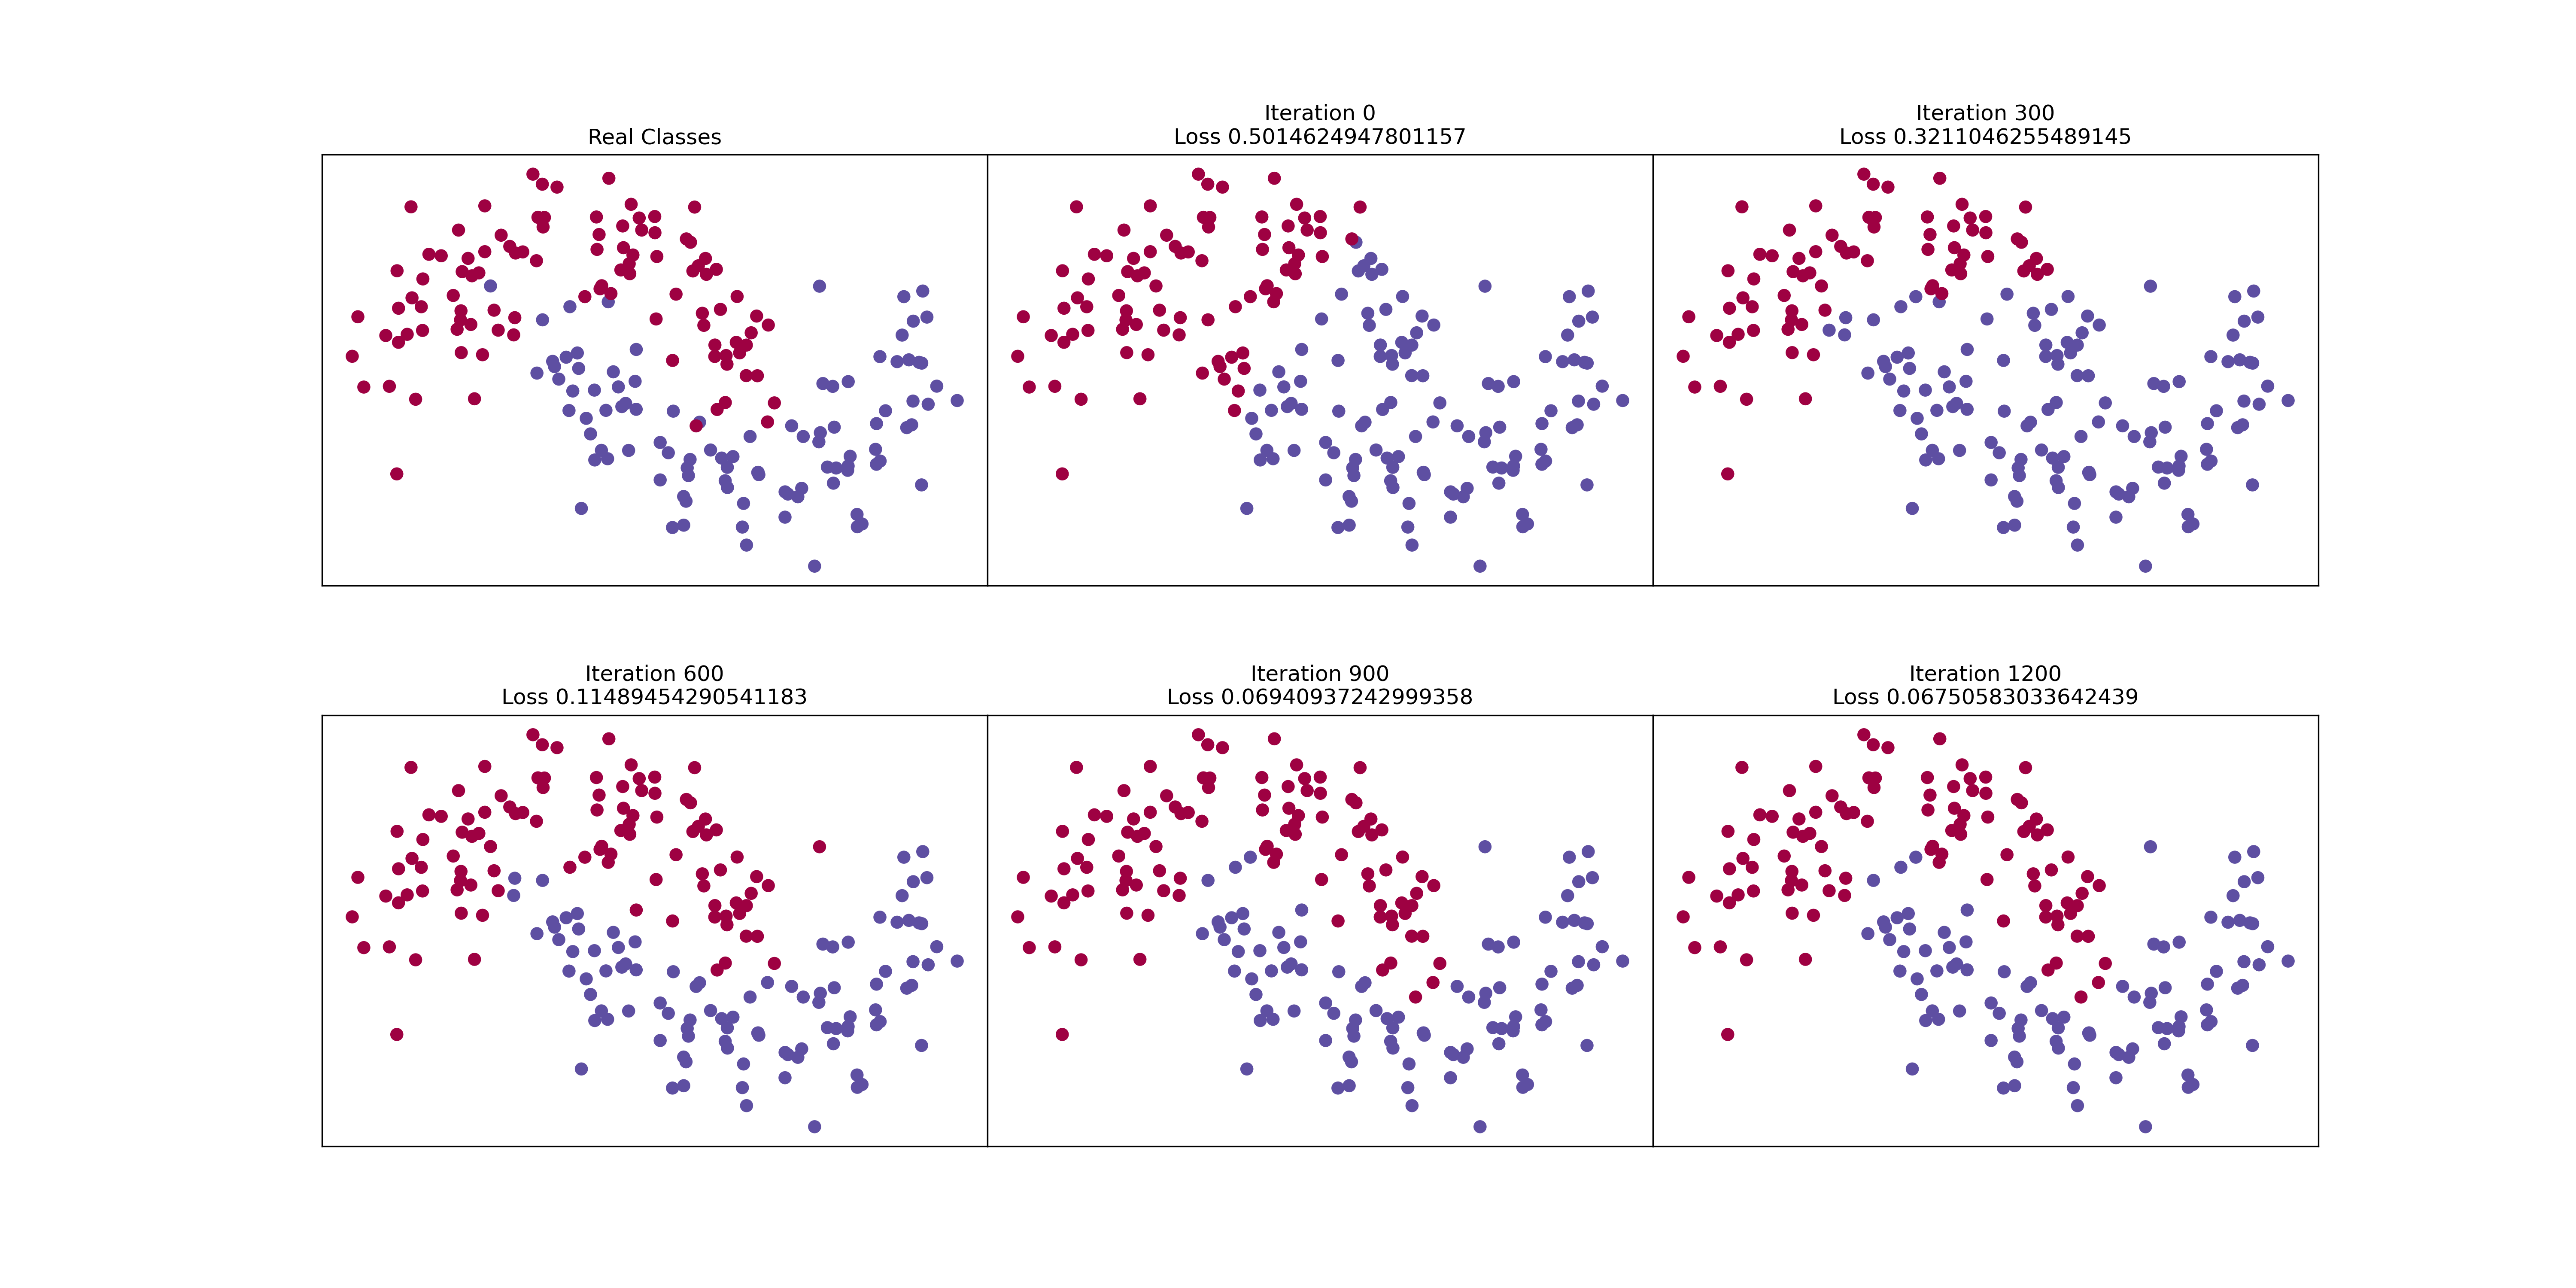
\includegraphics[width=\textwidth]{figs/1.png}
\end{center}

\subsection{تغییر تعداد نورون‌ها در لایه مخفی}
کد زیر در فایل
\texttt{2.py}
موجود است. در این کد در یک حلقه، هر بار شبکه عصبی را با تعداد متفاوتی نورون در لایه مخفی تعریف می‌کنیم و برای سنجیدن مدل از داده‌های
\texttt{test}
به جای
\texttt{train}
استفاده می‌کنیم.

\LTR
\lstinputlisting[language=Python]{2.py}
\RTL

خروجی به صورت زیر خواهد شد.

\begin{center}
    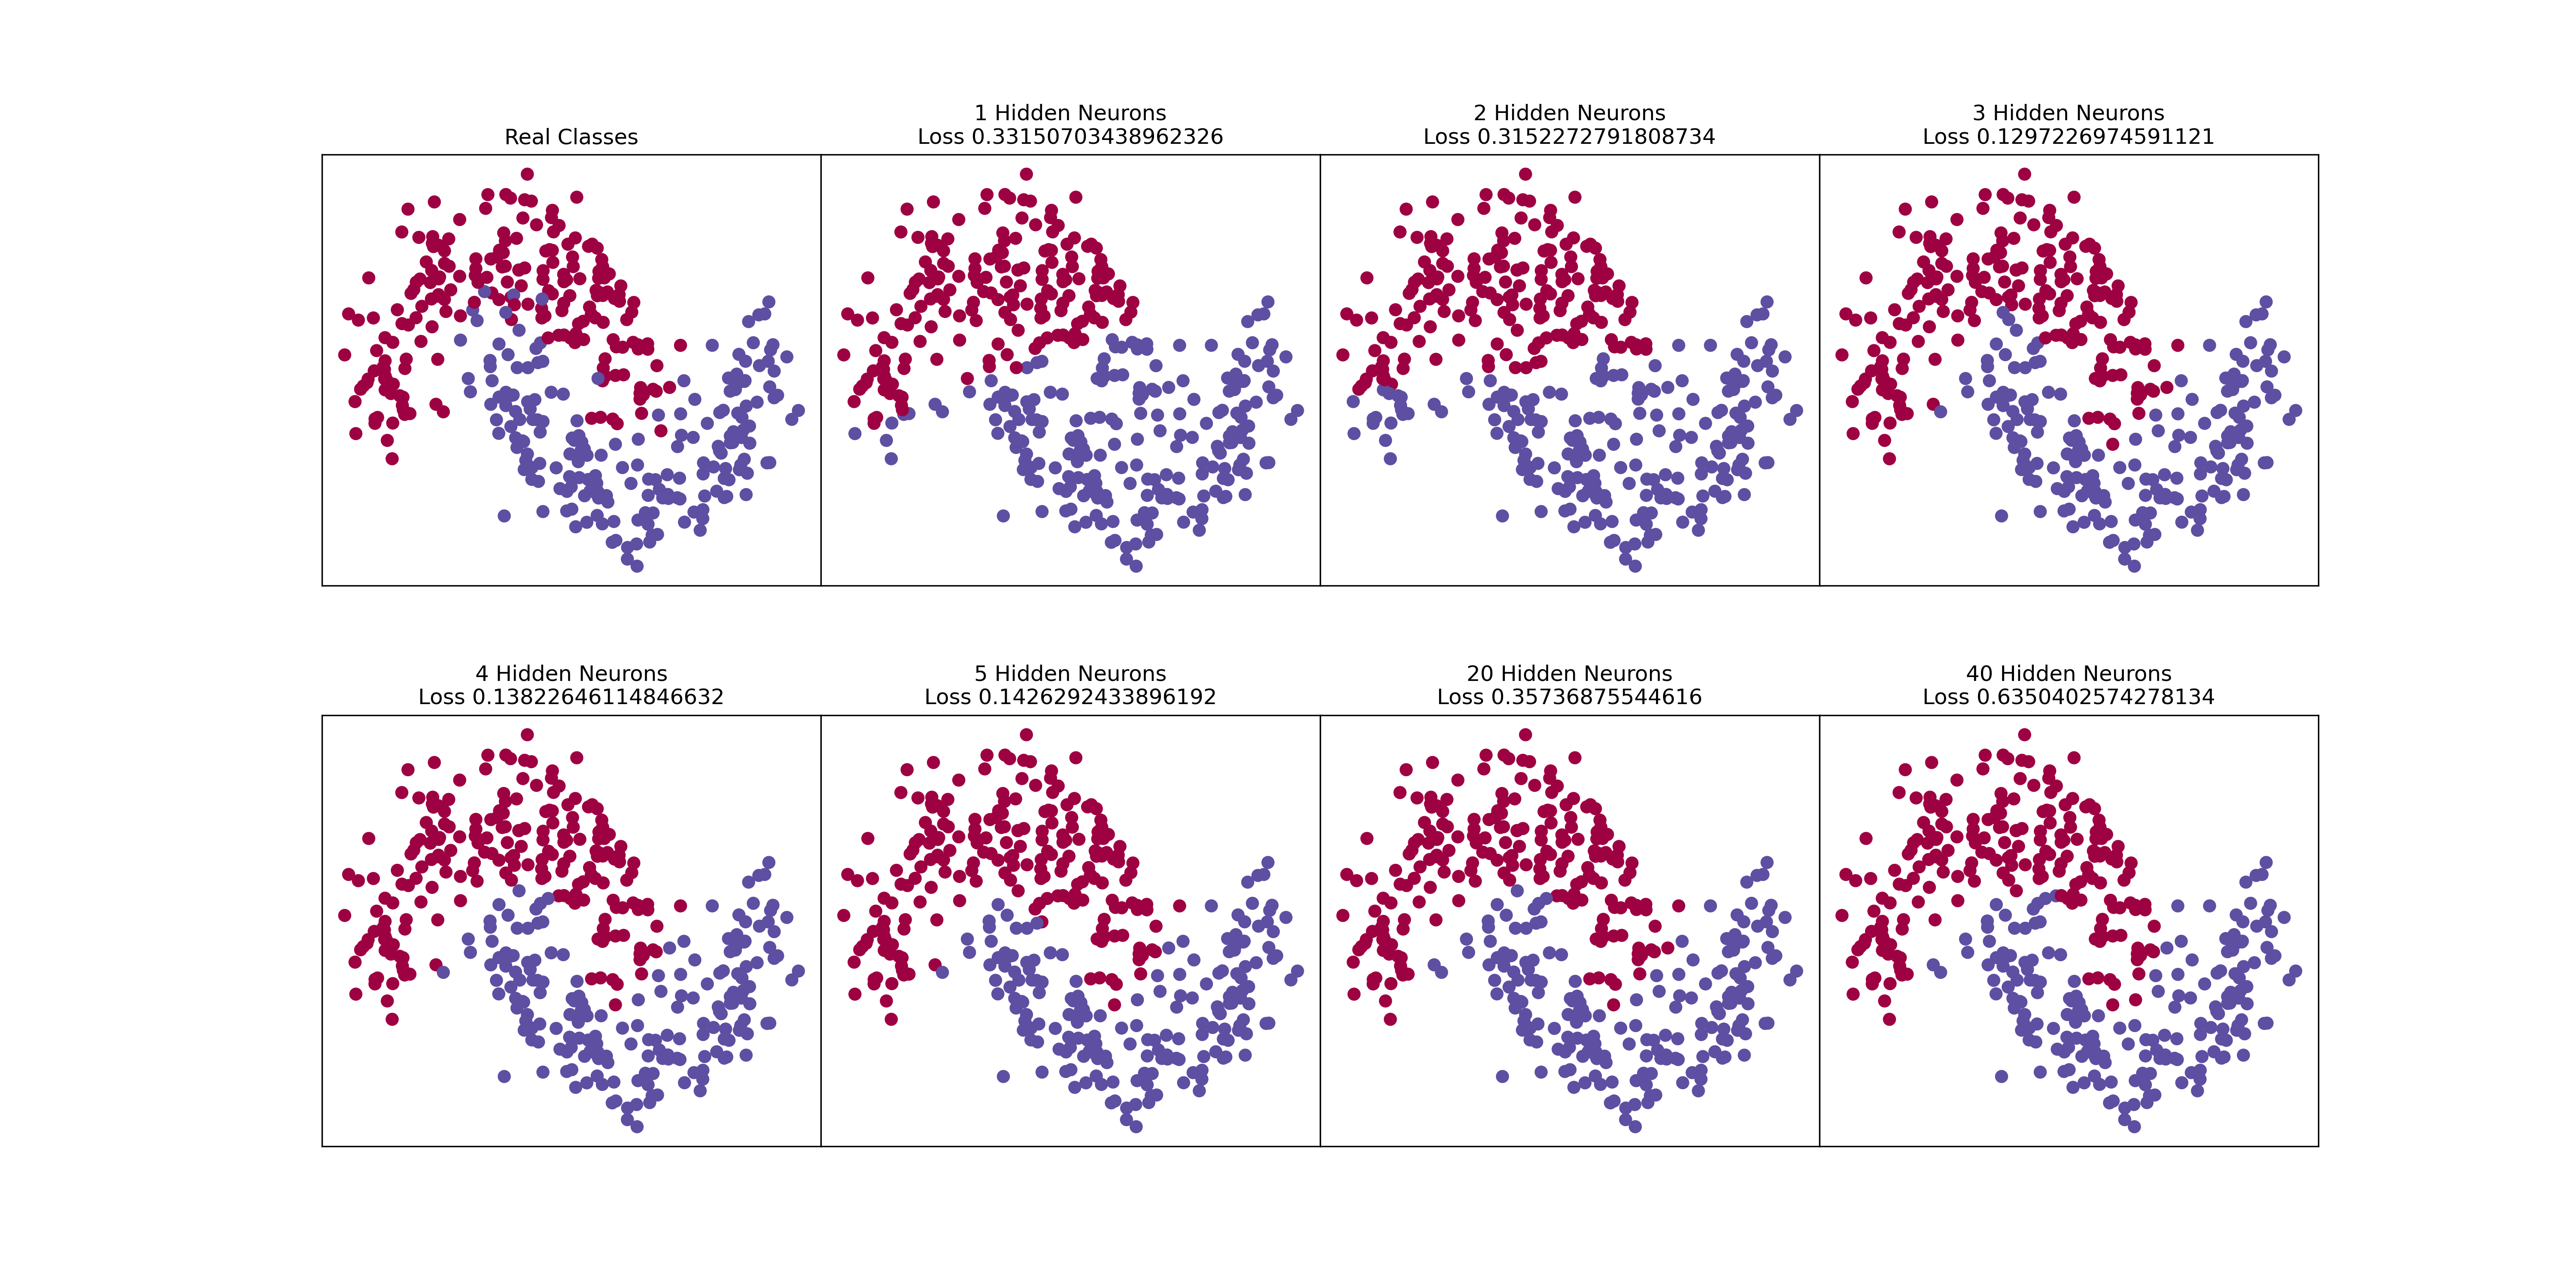
\includegraphics[width=\textwidth]{figs/2.png}
\end{center}

به نظر می‌رسد که همان سه نورون در لایه مخفی بهترین انتخاب باشد.

\subsection{استفاده از دسته‌های کوچک‌تر در آموزش شبکه}
کد زیر در فایل
\texttt{3.py}
موجود است. در این کد در یک حلقه، هر بار تعداد دسته‌ها را متفاوت در نظر می‌گیریم. مانند مورد قبل برای سنجیدن مدل از داده‌های
\texttt{test}
به جای
\texttt{train}
استفاده می‌کنیم.

\LTR
\lstinputlisting[language=Python]{3.py}
\RTL

خروجی به صورت زیر خواهد شد.

\begin{center}
    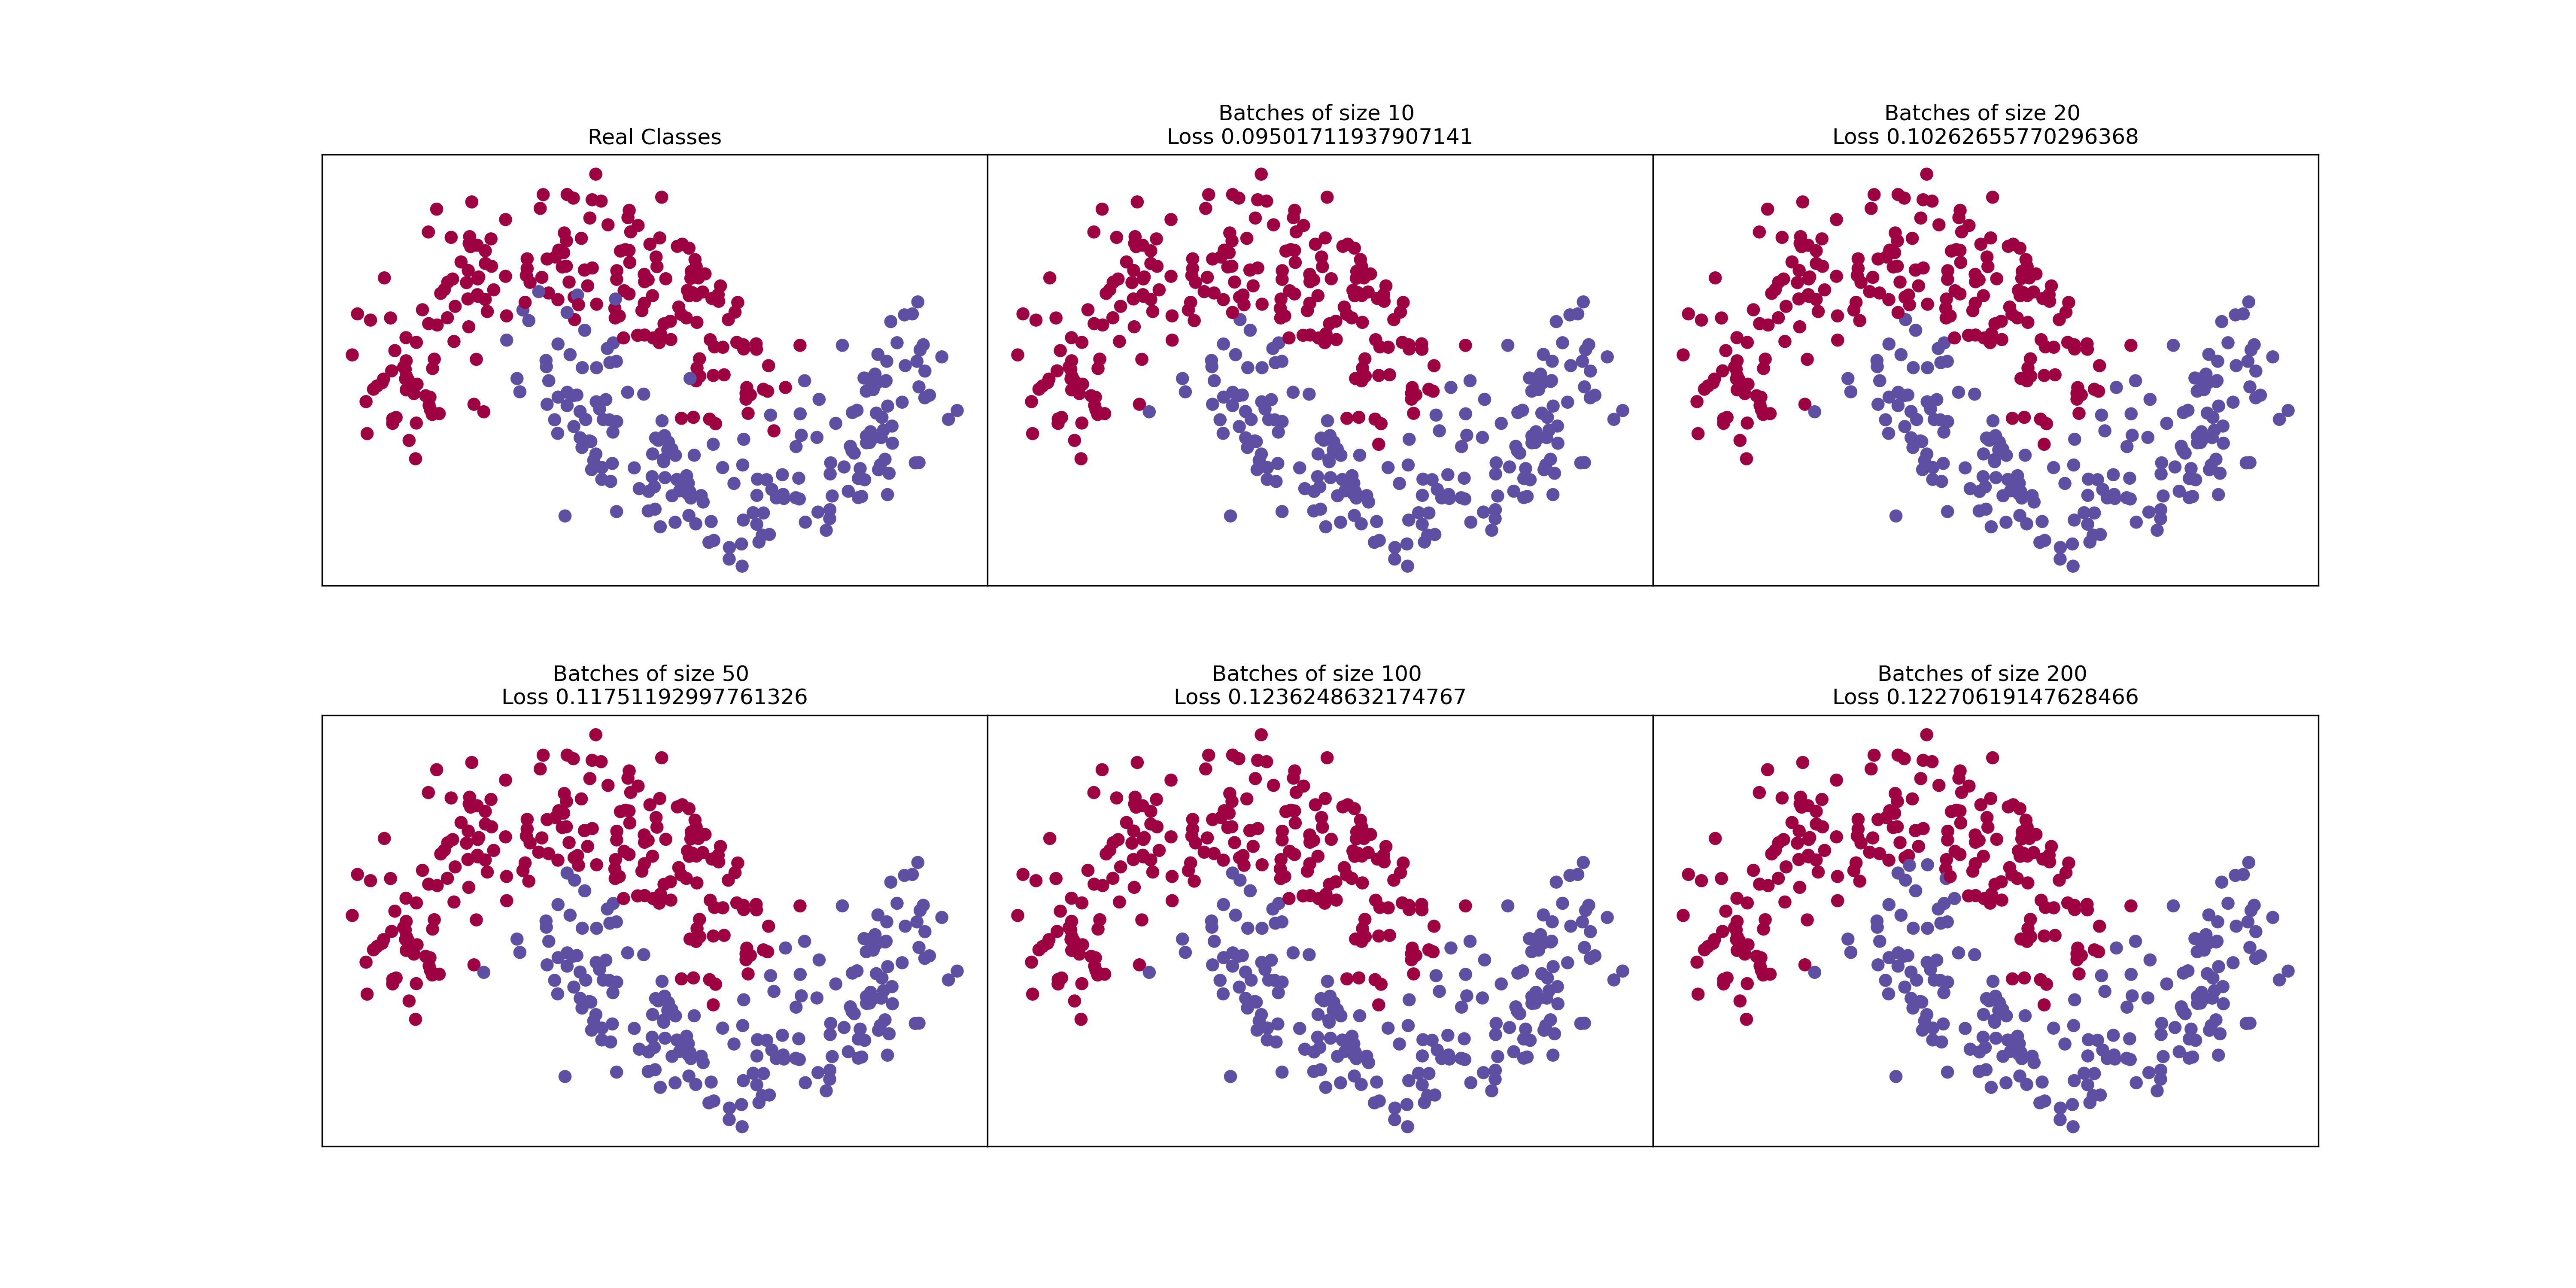
\includegraphics[width=\textwidth]{figs/3.png}
\end{center}

همانطور که در صورت پروژه آمده، به نظر می‌رسد استفاده از دسته‌های کوچک ۱۰-تایی خیلی بهتر از دسته کامل ۲۰۰-تایی عمل می‌کند.

\subsection{تبرید درجه یادگیری به تدریج}
کد زیر در فایل
\texttt{4.py}
موجود است. در این کد در یک حلقه، هر بار درجه تبرید را متفاوت در نظر می‌گیریم. مانند موارد قبل برای سنجیدن مدل از داده‌های
\texttt{test}
به جای
\texttt{train}
استفاده می‌کنیم.

\LTR
\lstinputlisting[language=Python]{4.py}
\RTL

خروجی به صورت زیر خواهد شد.

\begin{center}
    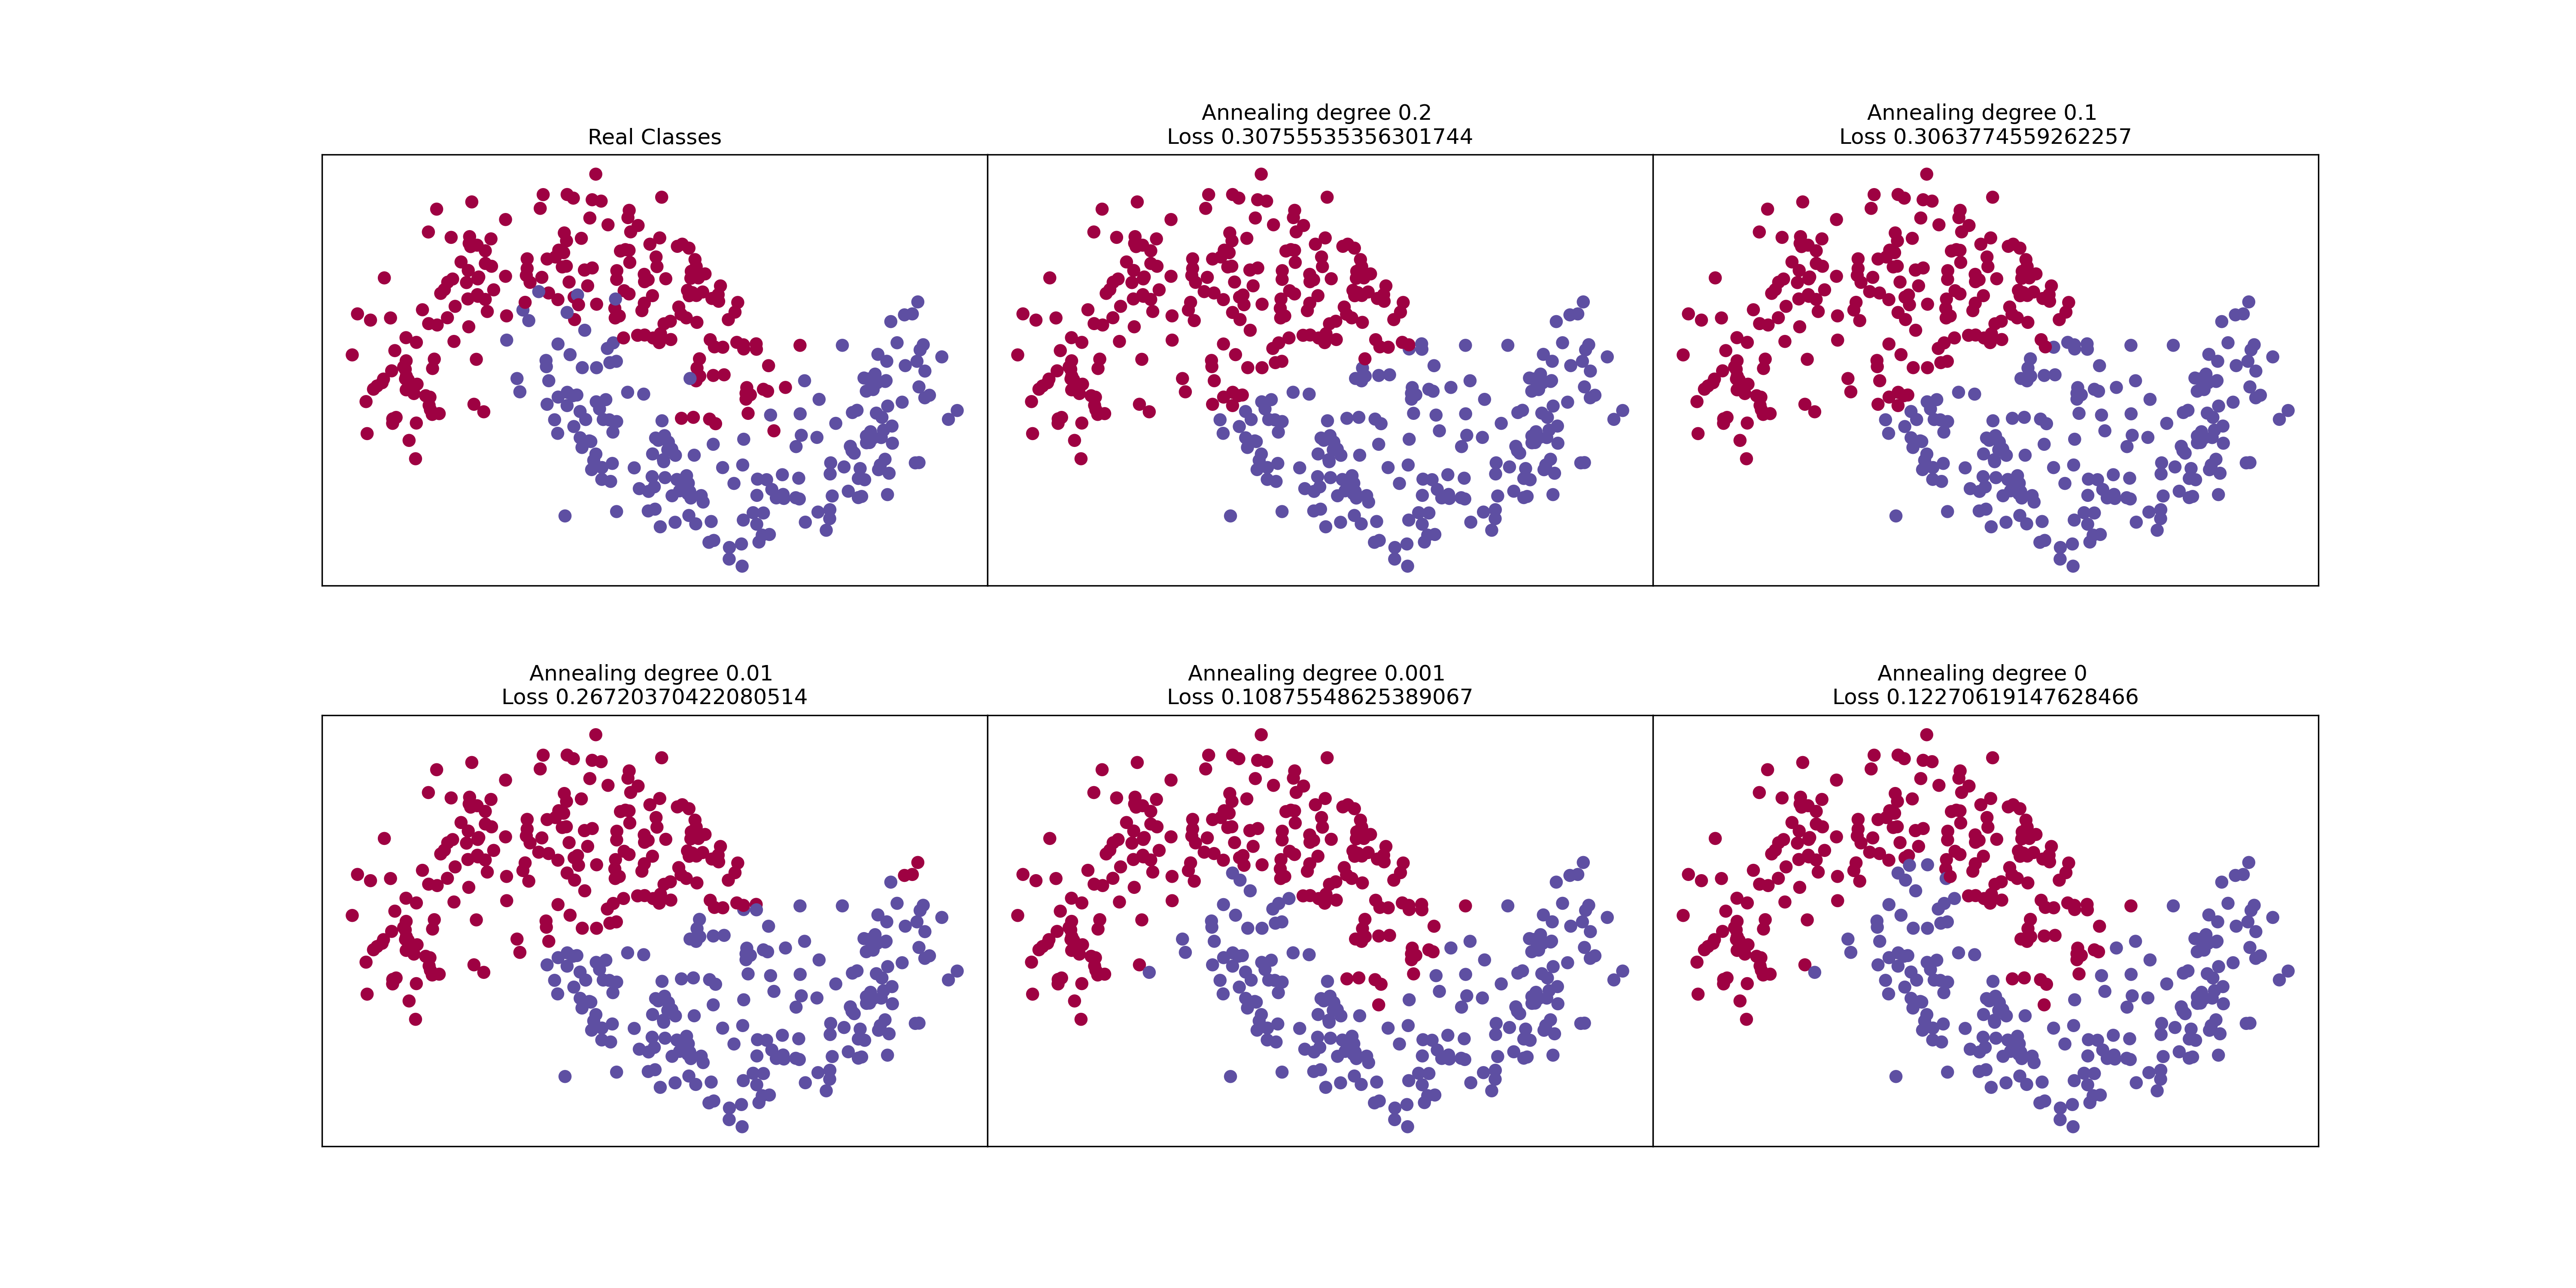
\includegraphics[width=\textwidth]{figs/4.png}
\end{center}

در حالاتی که درجه تبرید را بزرگ گرفتیم نتیجه از حالت معمولی با درجه صفر بدتر شده، اما می‌بینیم در حالتی که این درجه را خیلی کوچک و برابر
\lr{\texttt{0.001}}
در نظر گرفتیم نتیجه بهتری حاصل شده.

\subsection{تغییر تابع فعال‌سازی از \texttt{tanh} به \texttt{sigmoid}}
کد زیر در فایل
\texttt{5.py}
موجود است. در این کد یک بار با تابع فعال‌سازی
\texttt{tanh}
و بار دیگر با تابع فعال‌سازی
\texttt{sigmoid}
شبکه عصبی را ایجاد می‌کنیم (توابع و فرمول‌های مربوط به هر یک در بخش معرفی شبکه عصبی آمده.) و مانند موارد قبل برای سنجیدن مدل از داده‌های
\texttt{test}
به جای
\texttt{train}
استفاده می‌کنیم.

\LTR
\lstinputlisting[language=Python]{5.py}
\RTL

خروجی به صورت زیر خواهد شد.

\begin{center}
    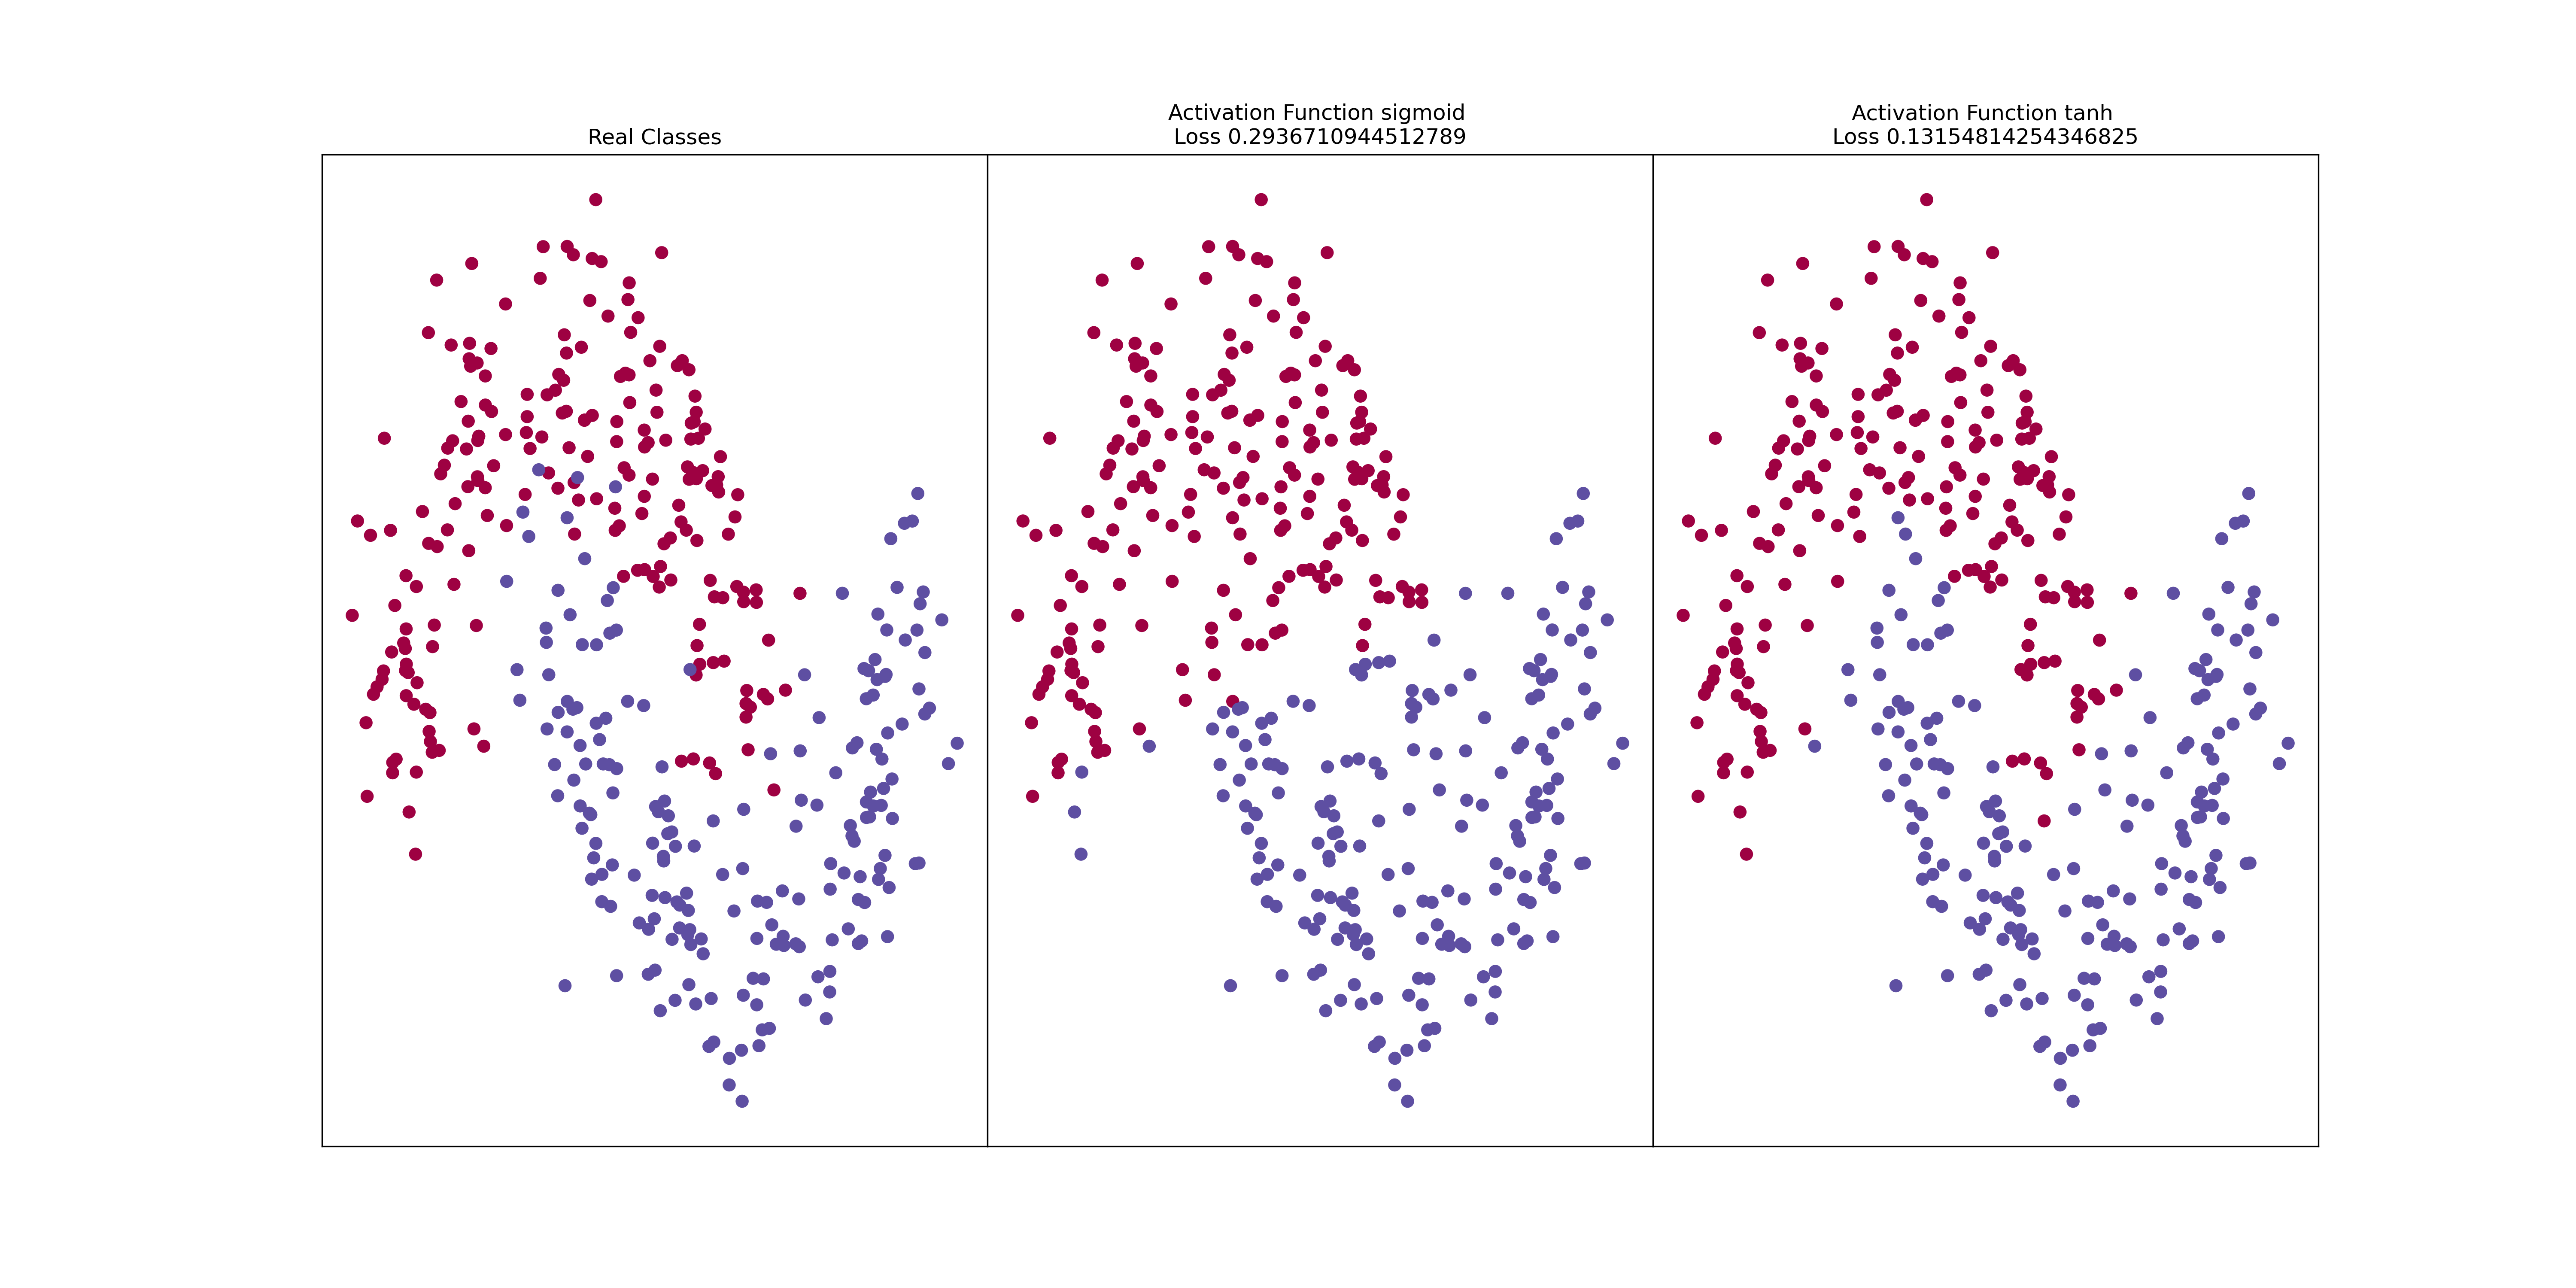
\includegraphics[width=\textwidth]{figs/5.png}
\end{center}

به نظر می‌رسد در این مسئله تابع
\texttt{tanh}
بهتر از
\texttt{sigmoid}
عمل می‌کند که با توجه به صورت پروژه همین انتظار می‌رود.

\subsection{داده‌هایی با سه کلاس به جای دو کلاس}
کد زیر در فایل
\texttt{6.py}
موجود است. در این کد داده‌هایی با سه کلاس تولید می‌کنیم که توضیح آن در بخش توابع کمکی آمده. مدل را آموزش می‌دهیم و مانند موارد قبل برای سنجیدن مدل از داده‌های
\texttt{test}
به جای
\texttt{train}
استفاده می‌کنیم.

\LTR
\lstinputlisting[language=Python]{6.py}
\RTL

خروجی به صورت زیر خواهد شد.

\begin{center}
    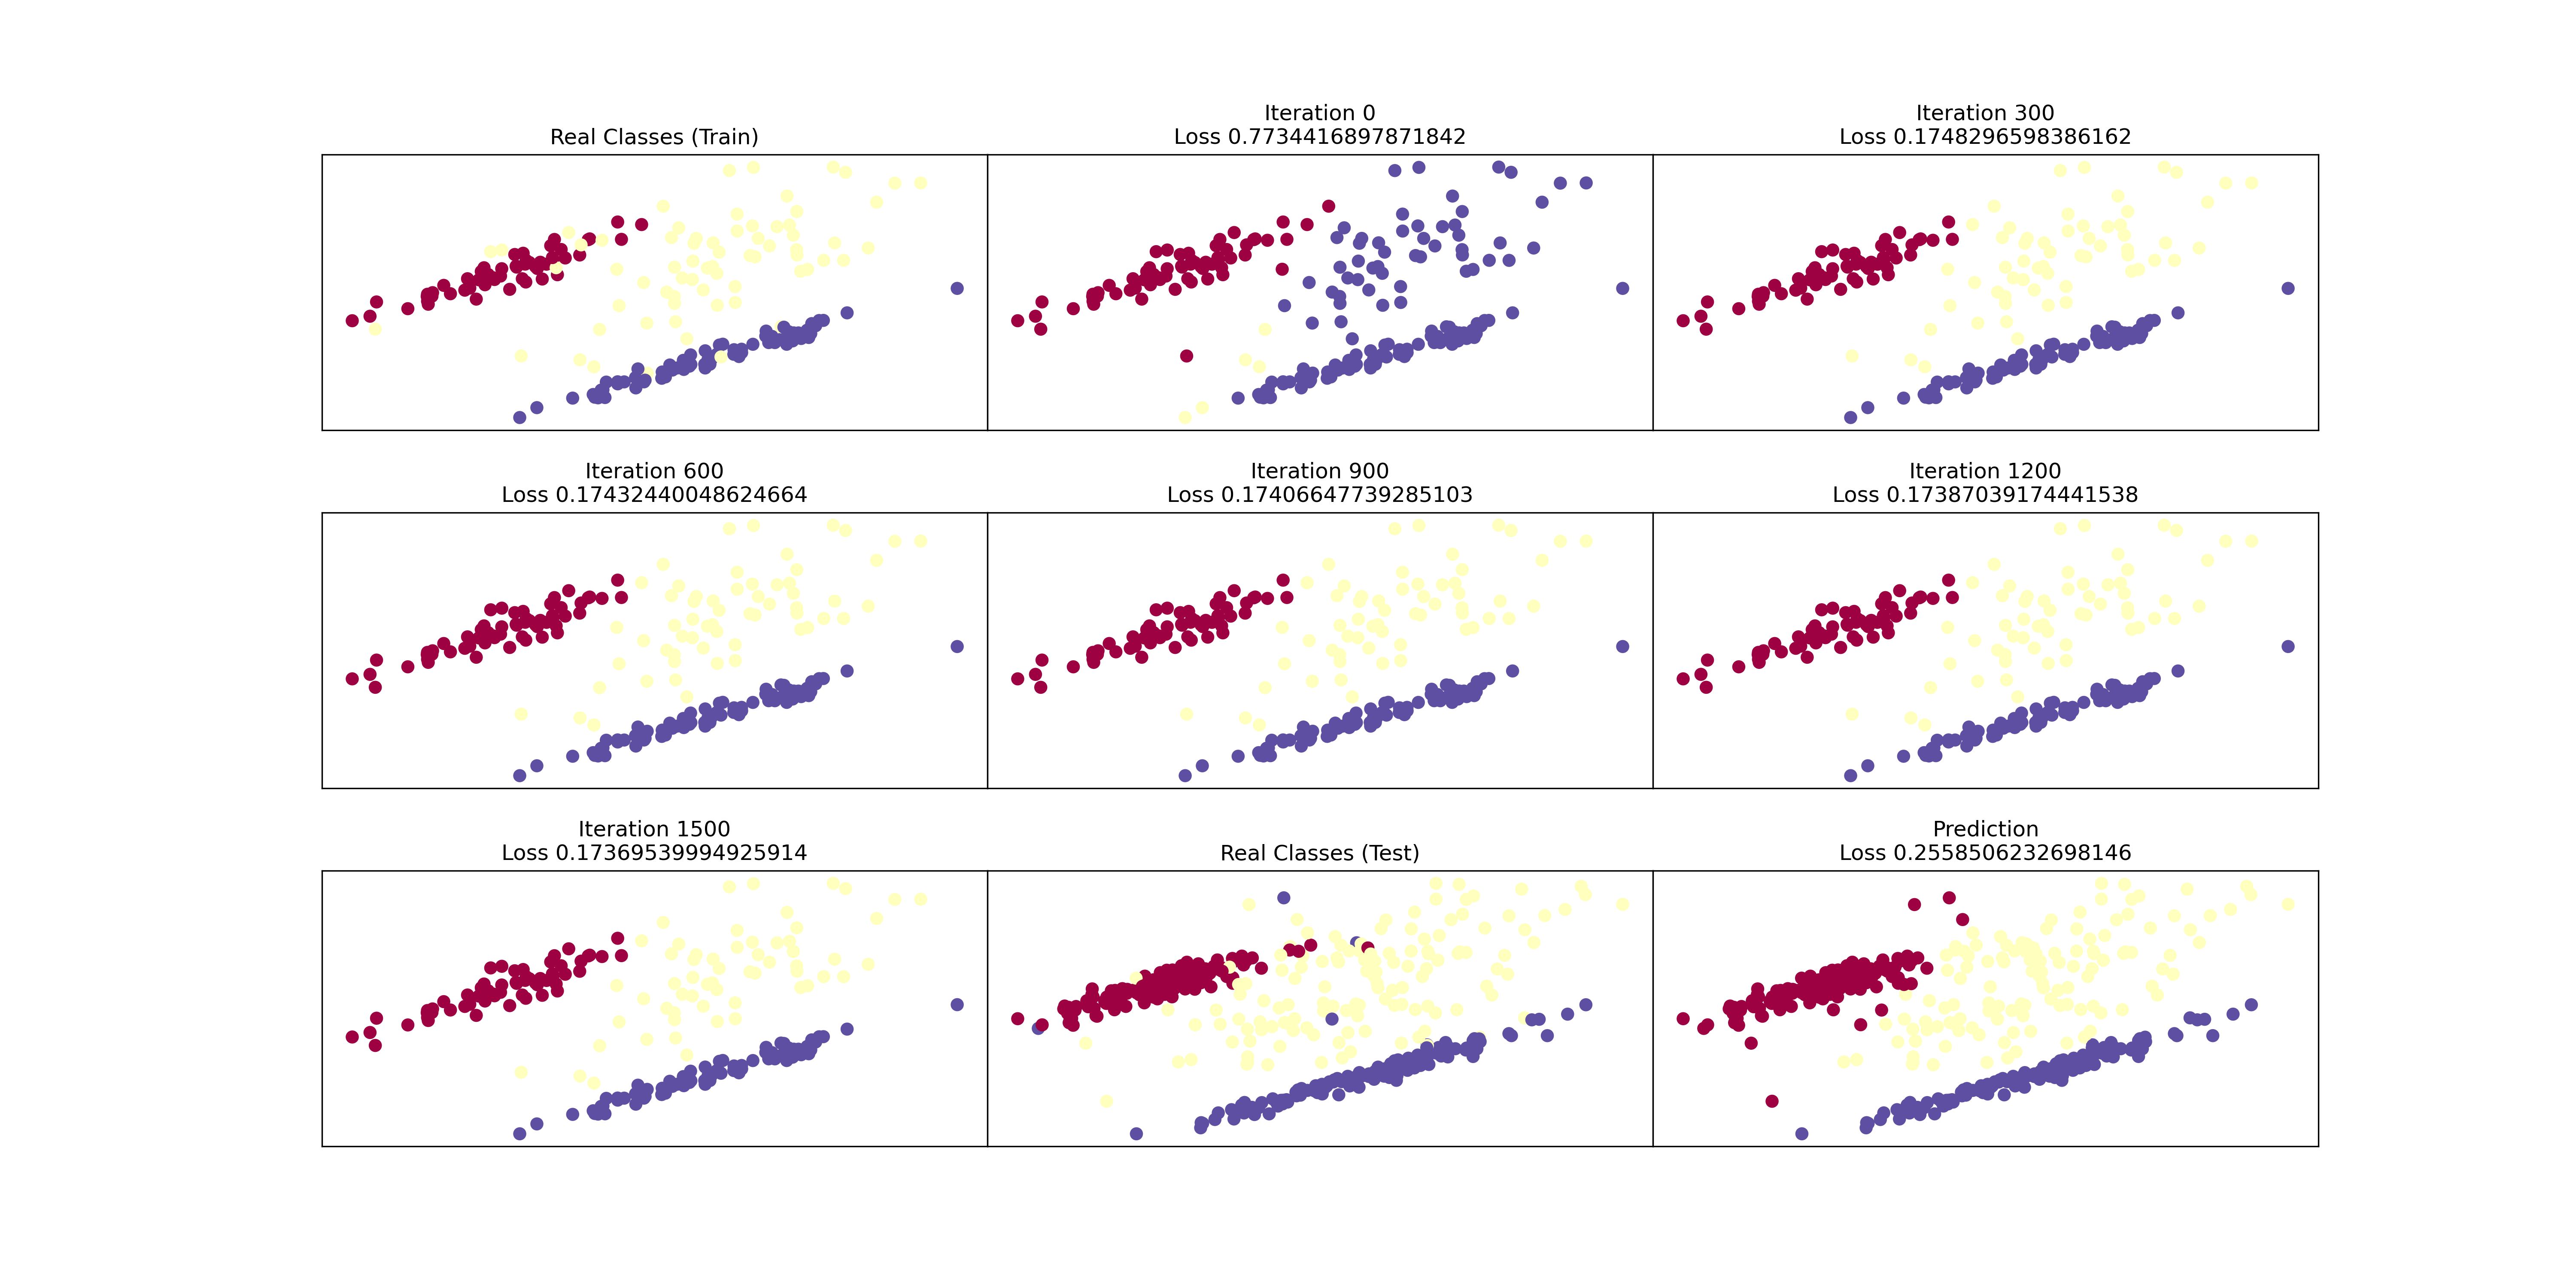
\includegraphics[width=\textwidth]{figs/6.png}
\end{center}

در تصویر بالا ترسیم‌هایی از مراحل آموزش مدل، داده‌های اصلی
\texttt{test}
و
\texttt{train}
و همچنین کلاس‌های پیش‌بینی‌شده برای داده
\texttt{test}
قابل رؤیت است.

\subsection{تغییر تعداد لایه‌های مخفی}
کد زیر در فایل
\texttt{7.py}
موجود است. در این کد در یک حلقه، هر بار لایه‌های مخفی را متفاوت در نظر می‌گیریم. مانند موارد قبل برای سنجیدن مدل از داده‌های
\texttt{test}
به جای
\texttt{train}
استفاده می‌کنیم.

\LTR
\lstinputlisting[language=Python]{7.py}
\RTL

خروجی به صورت زیر خواهد شد.

\begin{center}
    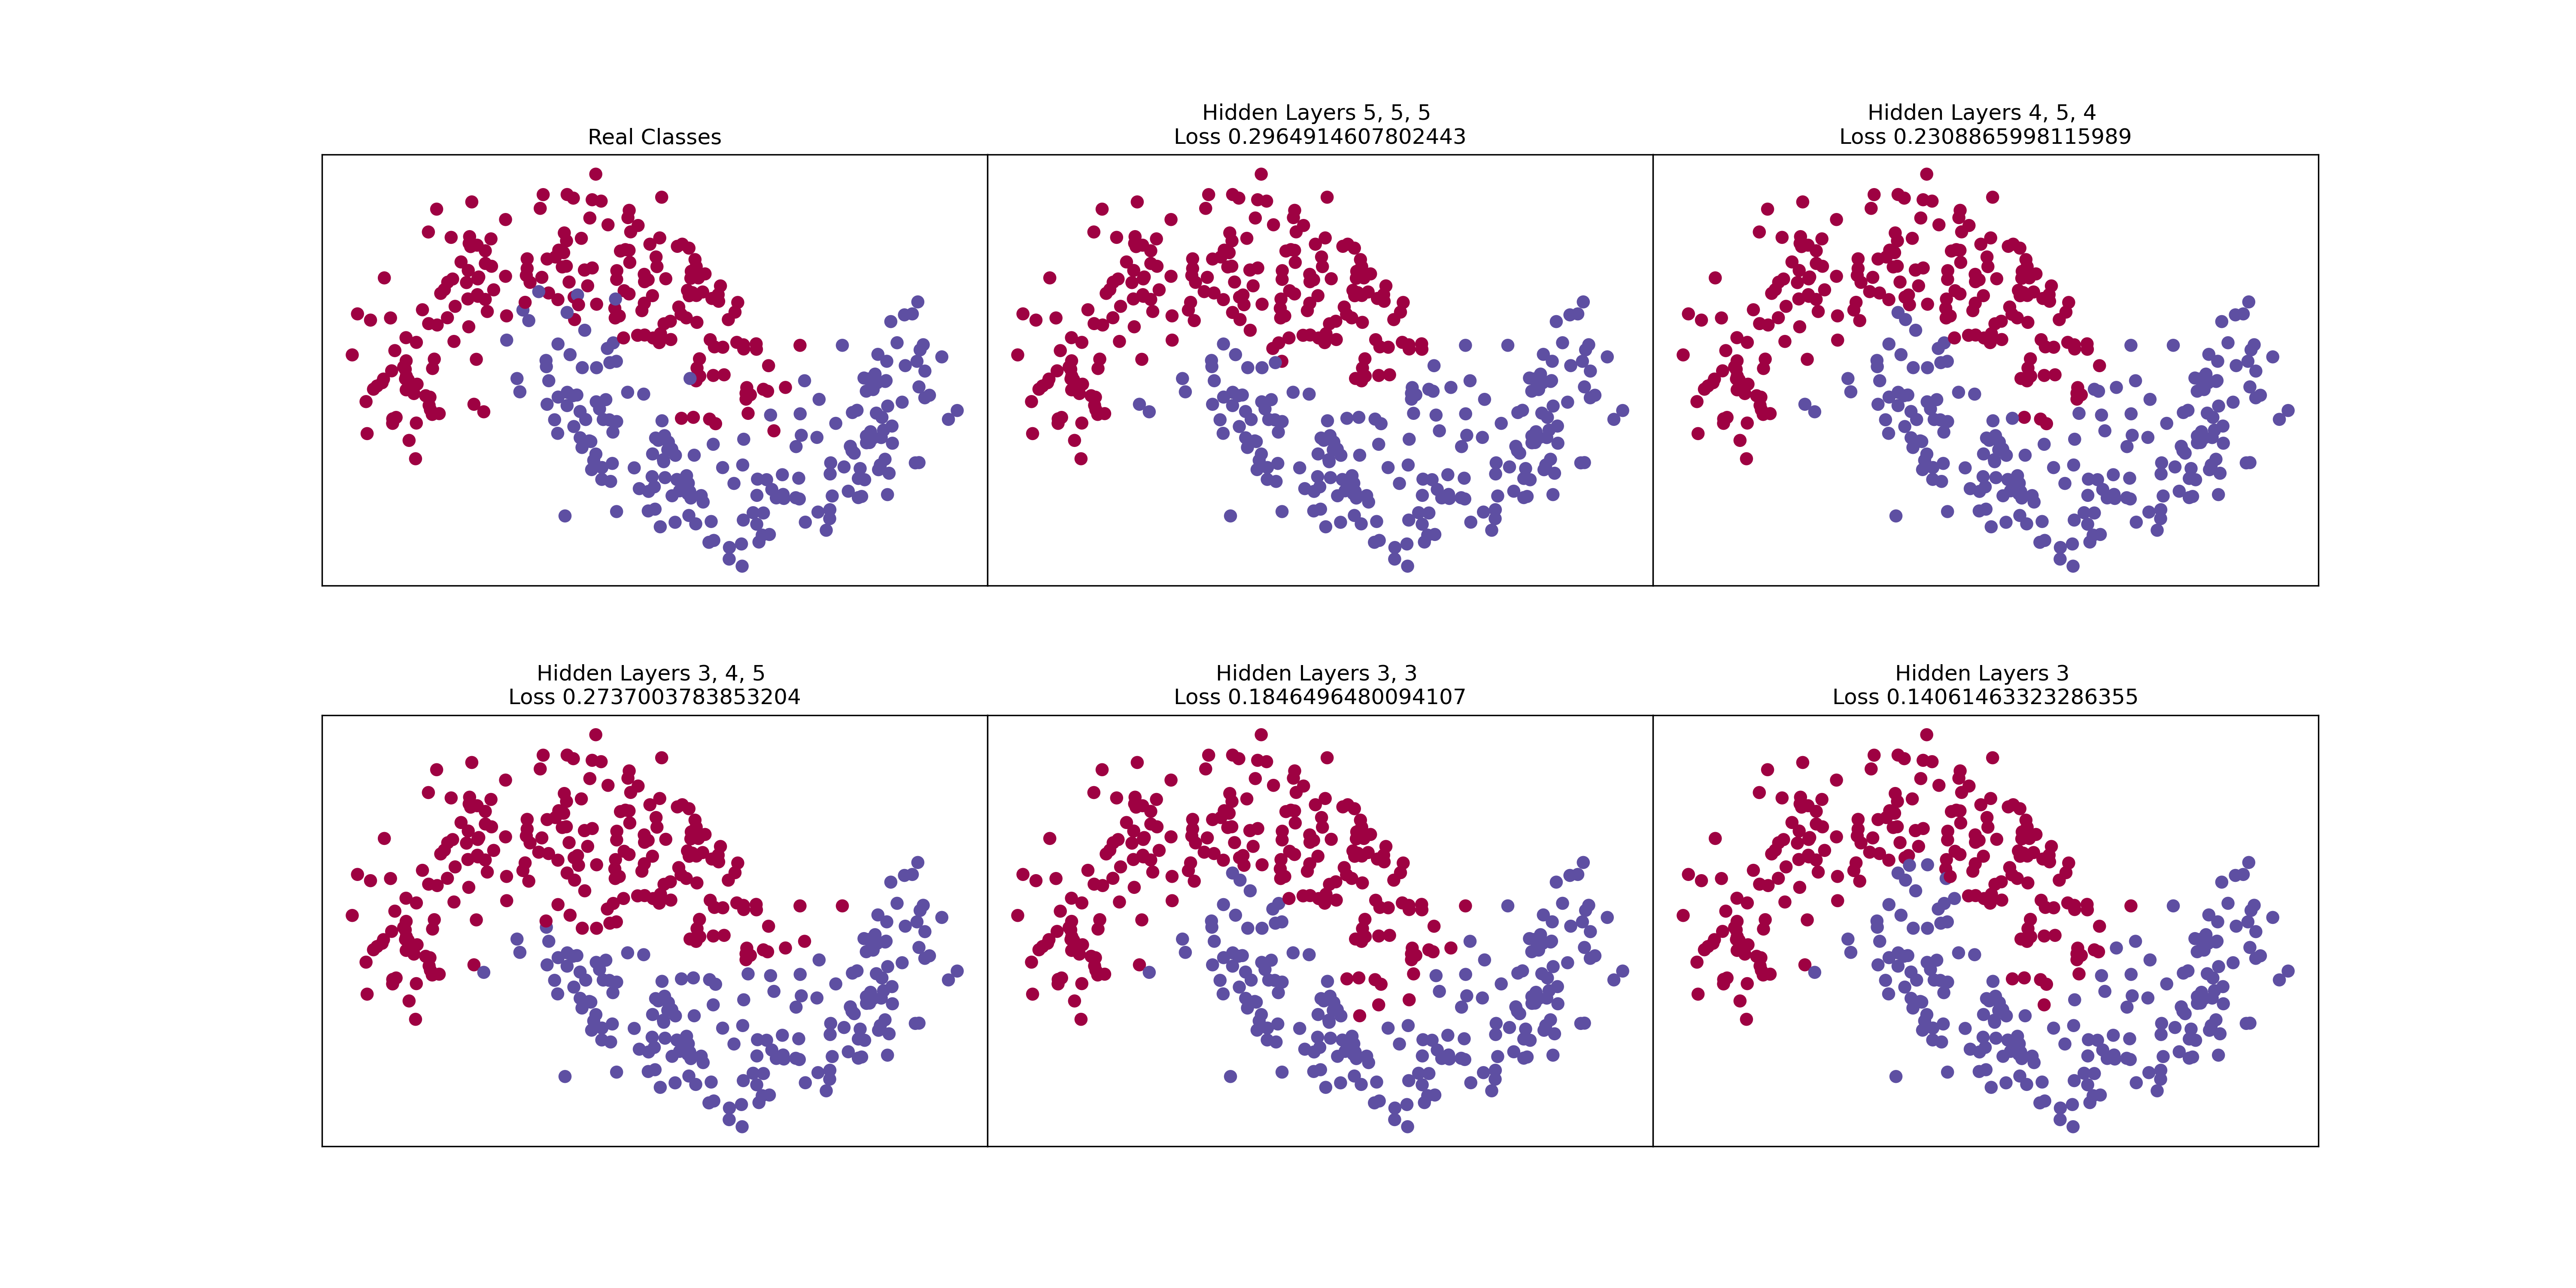
\includegraphics[width=\textwidth]{figs/7.png}
\end{center}

همانطور که در تصویر قابل‌مشاهده است به نظر می‌رسد همان یک لایه مخفی با سه نورون بهتر از سایر حالات عمل می‌کند.
\end{document}